\documentclass{book}
\title{A Computational Tour of Number Theory}
\author{Math 581f -- William Stein + students}

\usepackage{amsmath}
\usepackage{amssymb}
\usepackage{amsfonts}
\usepackage{amsthm}


%%%% Theoremstyles
\theoremstyle{plain}
\newtheorem{theorem}{Theorem}[section]
\newtheorem{proposition}[theorem]{Proposition}
\newtheorem{corollary}[theorem]{Corollary}
\newtheorem{claim}[theorem]{Claim}
\newtheorem{lemma}[theorem]{Lemma}
\newtheorem{hypothesis}[theorem]{Hypothesis}
\newtheorem{conjecture}[theorem]{Conjecture}

\theoremstyle{definition}
\newtheorem{definition}[theorem]{Definition}
\newtheorem{question}[theorem]{Question}
\newtheorem{idea}[theorem]{Idea}
\newtheorem{project}[theorem]{Project}
\newtheorem{problem}[theorem]{Problem}
\newtheorem{openproblem}[theorem]{Open Problem}
\newtheorem{challenge}[theorem]{Challenge}

%\theoremstyle{remark}
\newtheorem{goal}[theorem]{Goal}
\newtheorem{remark}[theorem]{Remark}
\newtheorem{remarks}[theorem]{Remarks}
\newtheorem{example}[theorem]{Example}
\newtheorem{exercise}[theorem]{Exercise}

\numberwithin{equation}{section}
\numberwithin{figure}{section}
\numberwithin{table}{section}


\usepackage{hyperref}  % so we have \url{...} command

\usepackage{sistyle}
\SIthousandsep{,}

\DeclareMathOperator{\Li}{Li}
\DeclareMathOperator{\Cl}{Cl}
\DeclareMathOperator{\ord}{ord}
\DeclareMathOperator{\realpart}{Re}

\newcommand{\C}{\mathbb{C}}
\newcommand{\Q}{\mathbb{Q}}
\newcommand{\Z}{\mathbb{Z}}
\newcommand{\F}{\mathbb{F}}
\renewcommand{\O}{\mathcal{O}}
\renewcommand{\Re}{\realpart}
\newcommand{\eps}{\varepsilon}


\usepackage{listings}
\lstdefinelanguage{Sage}[]{Python}
{morekeywords={True,False,sage,singular},
sensitive=true}
\lstset{
  showtabs=False,
  showspaces=False,
  showstringspaces=False,
  commentstyle={\ttfamily\color{dredcolor}},
  keywordstyle={\ttfamily\color{dbluecolor}\bfseries},
  stringstyle ={\ttfamily\color{dgraycolor}\bfseries},
  language = Sage,
  basicstyle={\scriptsize \ttfamily},
  aboveskip=1em,
  belowskip=1em,
  backgroundcolor=\color{lightyellow},
  frame=single
}

\usepackage{color}


\definecolor{lightyellow}{rgb}{1,1,.86}
\definecolor{dblackcolor}{rgb}{0.0,0.0,0.0}
\definecolor{dbluecolor}{rgb}{.01,.02,0.7}
\definecolor{dredcolor}{rgb}{0.8,0,0}
\definecolor{dgraycolor}{rgb}{0.30,0.3,0.30}
\definecolor{graycolor}{rgb}{0.35,0.35,0.35}

\usepackage{graphicx}


\newcommand{\hw}[2]{\par\vspace{1em}{\bf HW (#1):} {\em #2}\par\vspace{1em}}


\begin{document}
\maketitle
\tableofcontents

\chapter{Introduction: tour of the main questions}
In this book, we will explore several important central problems and
objects of number theory, and for each to explain how---in practice
(not just theory)---to {\em compute} with them.    Books,
papers, and web sites such as Wikipedia and Mathoverflow often
give excellent descriptions
of mathematical objects, algorithms, data, conjectures, and theorems.
However, they rarely give concrete instructions
so that you can manipulate them on a computer, with enough theoretical
discussion so that you understand the limitations and capabilities of
your tools.  That is the mission of the book you are looking at.


\section{Prime Numbers}
The prime numbers $2,3,5,7,11,\ldots, $ have fascinated
mathematicians for thousands of years.  Euclid proved there
are infinitely many: if $p_1,\ldots, p_n$ are primes,
then $p_1\cdots p_n + 1$ is an integer divisible by some
prime $p$ that isn't equal to any $p_i$.

Let's compute the primes up to 100:
\begin{lstlisting}
sage: prime_range(100)
[2, 3, 5, 7, 11, 13, 17, 19, 23, 29, 31, 37, 41, 43, 47, 53, 59, 61, 67, 71,
 73, 79, 83, 89, 97]
\end{lstlisting}
And draw a plot of the function $\pi(x)$ that counts the number of primes up to $x$ for $x<100$.
\begin{center}
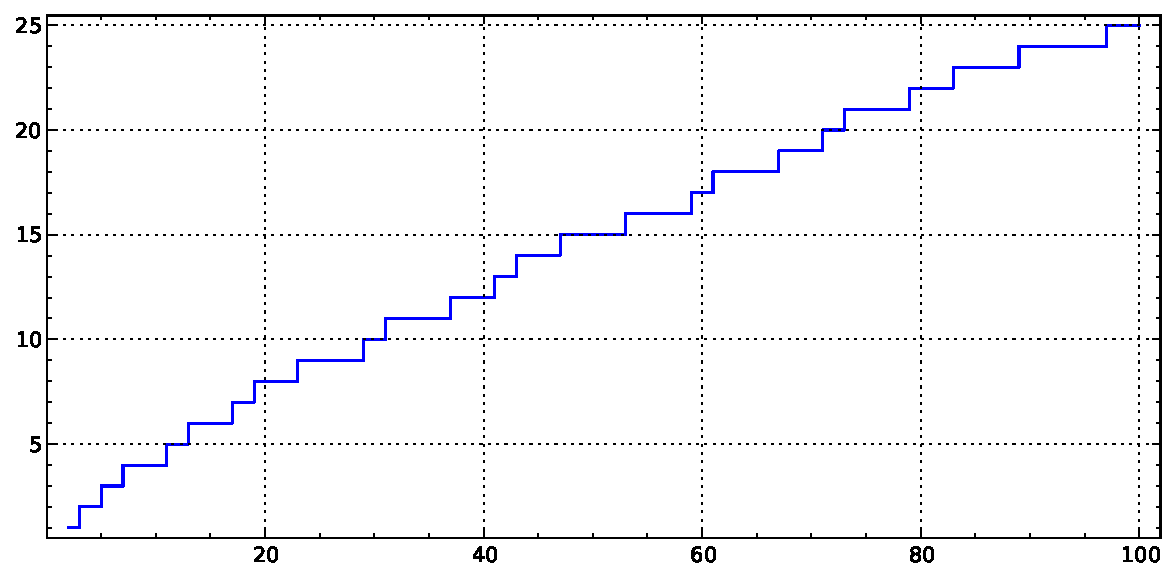
\includegraphics[width=.7\textwidth]{pics/prime_pi-2-100.pdf}
\end{center}

The {\em Prime Number Theorem}, which was proved over a century ago, asserts that $\pi(x) \sim x/\log(x)$:

\begin{lstlisting}
@interact
def f(B=[10^n for n in [2..9]]):
    show(plot(lambda x: prime_pi(x)/(x/log(x)), (x,2,B))
       + line([(0,1),(B,1)],color='red'))
\end{lstlisting}

\begin{center}
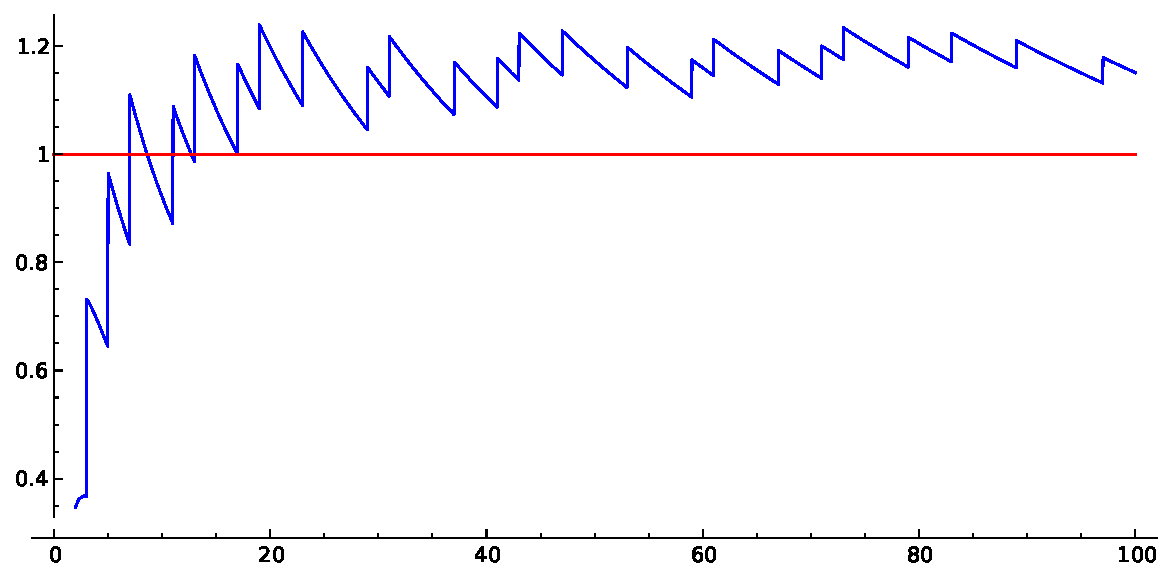
\includegraphics[width=.3\textwidth]{pics/pnt100.pdf}
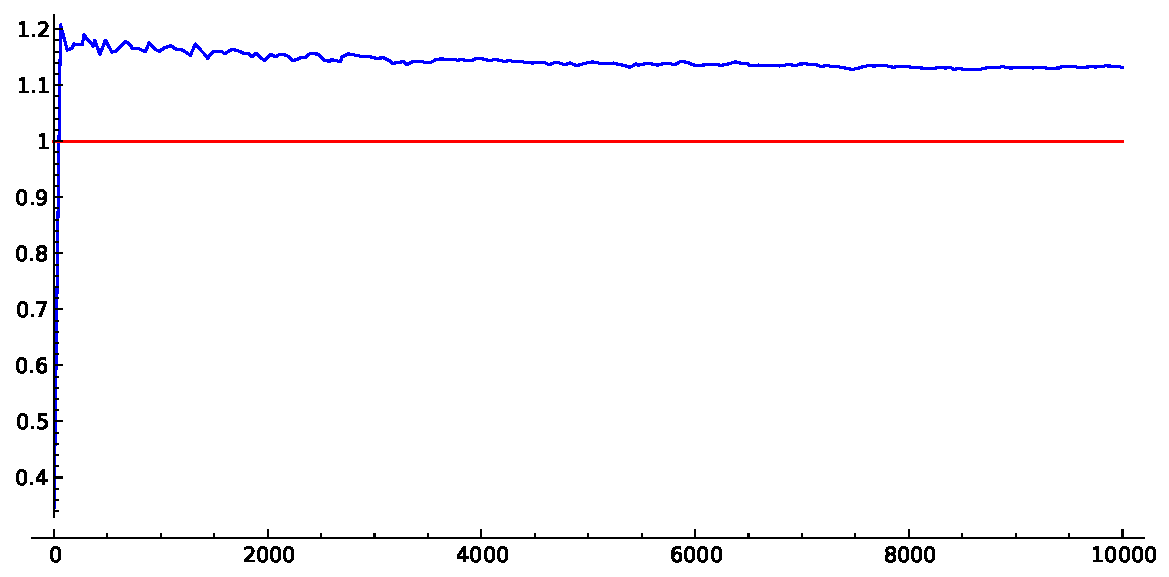
\includegraphics[width=.3\textwidth]{pics/pnt10000.pdf}
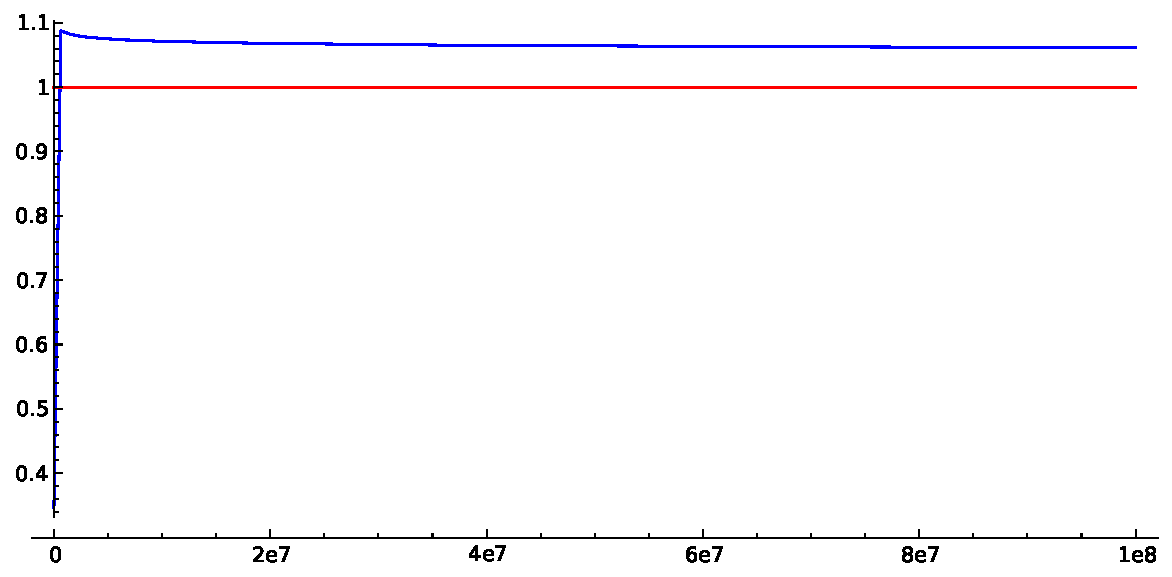
\includegraphics[width=.3\textwidth]{pics/pnt100000000.pdf}
\end{center}

The {\em Riemann Hypothesis}, which remains completely unsolved today,
asserts that for all $x\geq 2.01$,
$$
 |\pi(x) - \Li(x)| \leq \sqrt{x}\cdot \log(x),
$$
where
$$
 \Li(x) = \int_{2}^x \frac{dt}{\log(t)}
$$

In the range of the following plots, $\pi(x) - \Li(x)$ is
much smaller than $\sqrt{x}\log(x)$.
\begin{lstlisting}
@interact
def f(B=[10^n for n in [2..9]]):
    print "sqrt(B)*log(B) = ", round(sqrt(B)*log(B))
    show(plot(lambda x: prime_pi(x) - Li(x), (x,2,B)))
\end{lstlisting}
\begin{center}
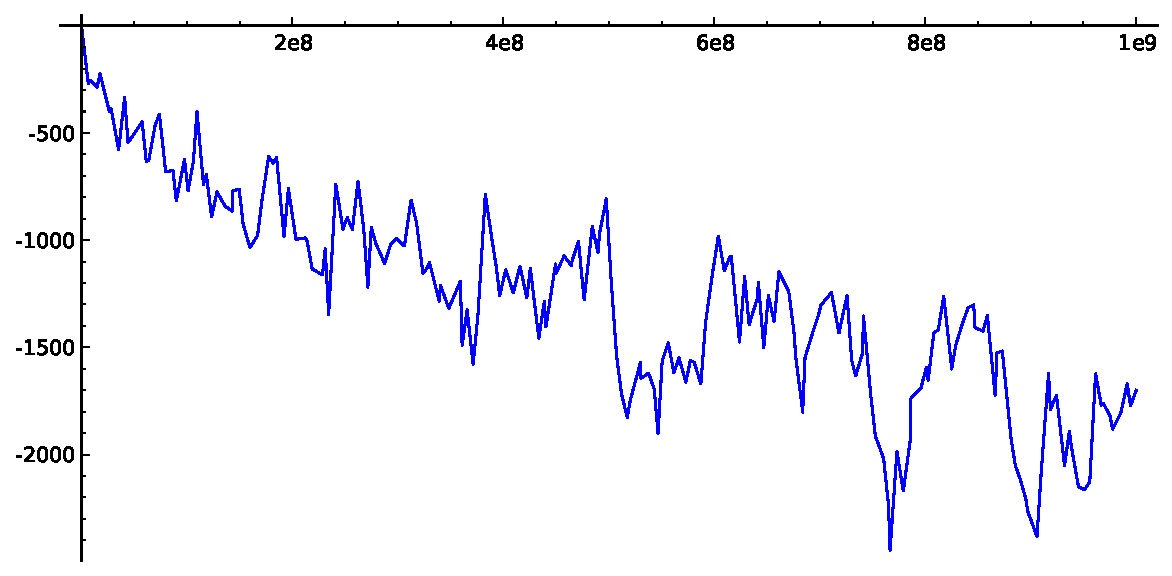
\includegraphics[width=.7\textwidth]{pics/pi_minus_li-1e9.pdf}
\end{center}
Up to $10^9$ we have $|\pi(x)-\Li(x)|$ is much
smaller than $\sqrt{10^9}\cdot \log(10^9) \sim  \num{655327}$.

\hw{Andrew and Bharath}{Can we prove anything toward $\sqrt{x}\cdot \log(x)$?}

\section{Class Numbers}
Number fields are a natural generalization of the rational numbers $\Q$,
to which ideas such as primes, and conjectures such as
the Riemann Hypothesis, etc., all generalize.  They have
been intensely studied, initially motivated by
work to prove Fermat's Last Theorem.

In this book we will assume you know abstract algebra; however,
as a quick reminder, an {\em ideal} $I$ in a commutative ring $R$ is an additive subgroup of $R$ such that for all $x\in R$ we have $xI \subset I$.
A {\em number field} $K$ is a finite algebraic extension of
the rational numbers $\Q$; equivalently, it is a field obtained
by adjoining a root $\alpha$ of some polynomial $f(x) \in \Q[x]$.
The {\em ring of integers} $R=\O_K$ of a number field $K$ is the
set of all $\alpha\in K$ such that $\alpha$ is a root of some
monic polynomial $f(x)\in\Z[x]$.  It is interesting to prove
that $R$ (as defined) is closed under addition and multiplication
(it is a ring).
In the special case when $K=\Q$, we have $R=\Z$.
\hw{Volunteer!}{Put a proof or good ref to proof in as a footnote.}

We can multiply any two nonzero ideals $I, J\subset R$ by taking
the ideal generated by all products of elements in $I$ with elements
in $J$.  With this operation, the set of nonzero ideals is an infinite
monoid (a group but without inverses).
For example, if $R=\Z$, then the nonzero ideals are in
bijection with positive integers, and the monoid is isomorphic to
$\Z_{>0}$ under addition.

An ideal $I$ is {\em principal} if there is some $\alpha \in R$ such
that $I = \{\alpha b : b \in R\}$, in which case we write $I=(\alpha)$.
Define an equivalence relation on nonzero ideals by
$I\sim J$ if $I=J\cdot (\alpha)$ for some principal ideal
$(\alpha)$.
The {\em class group} $\Cl(R)$ of $R$ is the quotient of the monoid of
nonzero ideals modulo this equivalence relation, i.e., modulo the
submonoid of principal ideals; it takes some work to show that
the result is an abelian {\em group}, i.e., every ideal class
has an inverse.

For example, if $R$ is a principal ideal domain (PID), i.e., if
every ideal is principal, then the class group is an abelian group
of order $1$.   In the following example, we consider $\Q(\sqrt{-2013})$.

\begin{lstlisting}
sage: K = QuadraticField(-2013); K
Number Field in a with defining polynomial x^2 + 2013
sage: C = K.class_group(); C
Class group of order 16 with structure C4 x C2 x C2 of Number Field in i
with defining polynomial x^2 + 2013
sage: C.gens()
(Fractional ideal class (41, i + 23), Fractional ideal class (47, i + 14),
 Fractional ideal class (2, i + 1))
sage: C.0 * C.1
Fractional ideal class (19, i + 1)
sage: (C.0)^4
Trivial principal fractional ideal class
\end{lstlisting}

One of the main theorems of algebraic number theory asserts that
for any number field $K$, the class group $\Cl(R)$ is a {\em finite}
abelian group.   This immediately suggests some basic questions.
For example, extending the computation above,
if we let $K$ vary over the imaginary quadratic fields
$K=\Q(\sqrt{d})$ with $d\leq -1$ square free, we obtain
a list of class numbers of these fields:
\begin{lstlisting}
sage: h = lambda d : QuadraticField(d).class_number()
sage: v = [h(-d) for d in [1..500] if is_squarefree(-d)]; v
[1, 1, 1, 2, 2, 1, 2, 1, 2, 4, 2, 4, 1, 4, 2, 3, 6, 6, 4, 3, 4, 4, 2, 2, 6,
4, 8, 4, 1, 4, 5, 2, 6, 4, 4, 2, 3, 6, 8, 8, 8, 1, 8, 4, 7, 4, 10, 8, 4, 5,
4, 3, 4, 10, 6, 12, 2, 4, 8, 8, 4, 14, 4, 5, 8, 6, 3, 6, 12, 8, 8, 8, 2, 6,
10, 10, 2, 5, 12, 4, 5, 4, 14, 8, 8, 3, 8, 4, 10, 8, 16, 14, 7, 8, 4, 6, 8,
10, 16, 1, 8, 10, 11, 12, 14, 12, 4, 8, 5, 10, 12, 8, 16, 12, 2, 4, 13, 4,
20, 4, 10, 9, 12, 6, 4, 8, 20, 20, 8, 3, 8, 6, 14, 8, 10, 4, 16, 12, 7, 8,
5, 10, 20, 12, 12, 2, 12, 8, 15, 12, 12, 6, 12, 7, 4, 16, 12, 16, 8, 4, 6,
13, 8, 20, 2, 22, 11, 8, 12, 6, 14, 20, 8, 3, 16, 12, 14, 20, 4, 18, 8, 6,
8, 8, 12, 10, 16, 3, 12, 8, 19, 8, 26, 10, 12, 10, 20, 8, 4, 22, 12, 24, 8,
3, 12, 18, 8, 6, 28, 8, 10, 5, 14, 16, 16, 4, 8, 6, 19, 18, 20, 12, 9, 12,
8, 10, 28, 16, 3, 20, 8, 17, 8, 20, 22, 16, 14, 12, 10, 8, 6, 20, 16, 20,
16, 2, 16, 16, 16, 16, 6, 20, 10, 12, 8, 9, 10, 10, 24, 2, 16, 12, 21, 12,
24, 4, 20, 8, 15, 8, 5, 8, 32, 14, 20, 6, 12, 14, 20, 8, 26, 30, 8, 7, 16,
8, 7, 16, 20, 16, 12, 20, 8, 25, 16, 20, 4, 20, 7, 20, 9, 12, 28, 24, 8, 3]
\end{lstlisting}
Looking at this list, it is natural to guess that $1$ occurs only finitely
many times -- in fact, Gauss noticed that $1$ only appears 9 times:
\begin{lstlisting}
sage: v.count(1)
9
\end{lstlisting}
and {\em conjectured} that the corresponding $9$ fields are the only
quadratic imaginary fields with class number $1$.
Heegner (and independently, Stark) later proved this conjecture.
Also, deep work of Goldfeld and Gross-Zagier involving elliptic
curve $L$-functions, yielded an algorithm to find all quadratic
imaginary fields with given class number, which Mark Watkins has made
much more efficient in his thesis work.  (The crucial input here
was a proof that if $E$ is the elliptic curve $y^2 + y = x^3 - 7x + 6$,
then $\ord_{s=1}L(E,s)=3$, where $L(E,s)$ is the $L$-series
of $E$.)

What about the other direction: positive $d$?
\begin{lstlisting}
sage: h = lambda d : QuadraticField(d).class_number()
sage: v = [h(d) for d in [2..500] if is_squarefree(d)]; v
[1, 1, 1, 1, 1, 2, 1, 1, 1, 2, 1, 1, 1, 1, 1, 2, 1, 2, 1, 1, 2, 2, 1, 1,
2, 1, 2, 1, 1, 1, 2, 1, 2, 1, 2, 1, 1, 1, 2, 2, 1, 1, 2, 1, 1, 2, 1, 2,
3, 4, 1, 2, 1, 2, 1, 2, 1, 1, 2, 1, 1, 2, 1, 2, 2, 1, 1, 2, 2, 1, 2, 2,
1, 2, 2, 2, 1, 1, 4, 1, 1, 1, 1, 2, 1, 1, 3, 2, 4, 2, 1, 1, 2, 2, 1, 1,
2, 1, 1, 2, 1, 1, 4, 1, 2, 1, 2, 1, 1, 2, 2, 2, 2, 2, 2, 1, 1, 2, 4, 1,
1, 1, 2, 2, 2, 1, 1, 4, 1, 1, 1, 2, 1, 2, 4, 2, 2, 3, 8, 1, 3, 2, 4, 1,
6, 1, 2, 1, 1, 2, 2, 1, 1, 1, 3, 4, 3, 2, 2, 1, 1, 2, 2, 2, 1, 1, 2, 4,
1, 1, 1, 2, 1, 2, 2, 2, 4, 4, 1, 2, 2, 2, 1, 1, 2, 2, 1, 1, 2, 1, 1, 2,
1, 2, 2, 3, 4, 4, 3, 2, 1, 4, 1, 1, 2, 1, 2, 1, 2, 6, 1, 1, 1, 2, 2, 2,
1, 3, 2, 2, 2, 1, 4, 2, 1, 2, 2, 1, 1, 1, 1, 2, 2, 1, 4, 2, 1, 2, 2, 1,
1, 8, 5, 2, 2, 2, 2, 1, 4, 2, 1, 2, 1, 2, 1, 1, 1, 2, 6, 2, 2, 1, 1, 4,
4, 1, 4, 5, 8, 3, 4, 1, 2, 1, 2, 1, 1, 4, 1, 2, 1, 4, 1, 2, 2, 1, 3, 2,
2, 3, 2, 1, 1, 2, 2, 4, 2, 1, 1, 1, 2, 2, 1, 2, 5]
sage: v.count(1)
141
\end{lstlisting}
It's natural to guess that there there are infinitely many
real quadratic fields with class number $1$.
This is an unsolved problem, though it is supported
by the Cohen-Lenstra heuristics.   In fact, even proving
that there are infinitely many number fields (not just quadratic
fields) with class number $1$ is an unsolved problem.

\hw{Volunteer}{What proportion of real quadratic fields are
predicted to have class number $1$?}

\section{Fermat's Last Theorem}\label{sec:fltintro}
Fermat's Last Theorem -- a problem from the 1600s! -- asserts
that whenever $n\geq 3$, then there are no positive integer
solutions to the Diophantine equation
$$
X^n + Y^n = Z^n.
$$
This seemingly approachable problem has a long and colorful
history.
When $n=3$ the equation is
$$
X^3 + Y^3 = Z^3,
$$
which is the (projective homogenous) equation of the plane cubic algebraic
curve $x^3 + y^3 = 1$:
\begin{lstlisting}
%var x y
implicit_plot(x^3 + y^3 == 1, (x,-2,2), (y,-2,2))
\end{lstlisting}
\begin{center}
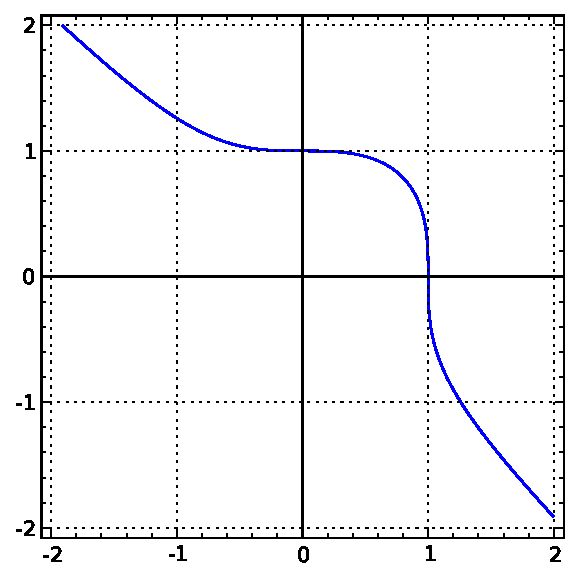
\includegraphics[width=.5\textwidth]{pics/flt3.pdf}
\end{center}
This is an example of an elliptic curve; you should
see some rational points on it---namely $(1,0)$ and $(0,1)$---these
correspond to torsion points on the elliptic curve, and to solutions
to the Fermat equation with $X$ or $Y$ equal to $0$.

For general $n\geq 5$, Fermat's assertion was finally resolved by much modern
work in number theory, culminating with a major theorem of
Andrew Wiles.  The basic strategy, which is useful for
attacking a wide range of Diophantine equations, is as follows.
Given a specific counterexample
$a^n + b^n = c^n$ to Fermat's claim (with say $n$ prime), we associate
an elliptic curve (the ``Frey curve'')
$$
  E: \quad y^2 = x(x-a^n)(x+b^n).
$$
By counting solutions modulo $p$ to the equation that defines this curve (or
any nonsingular curve of the form $y^2=x^3+\alpha x + \beta$ for that matter),
we define an $L$-series
$$
L(E,s) =
\prod_{p \text{ prime}} \frac{1}{1-a_p p^{-s} + \varepsilon(p)\cdot p^{1-2s}}
 = \sum_{n\geq 1} \frac{a_n}{n^s},
$$
where $\varepsilon(p)=1$ if $p\nmid abc$ and $\varepsilon(p)=0$ otherwise,
and $a_p = p+1-\#E(\F_p)$.
Old work of Hasse (and others)
shows that this $L$-series defines a complex analytic
function on some right half plane; people then conjectured (and
subsequently proved!)
that $L(E,s)$ extends to a holomorphic function on all $\C$.
Birch and Swinnerton-Dyer even went so far as to conjecture
that most everything about the arithmetic of $E$
is determined by the leading coefficient of the
Taylor expansion of $L(E,s)$ about $s=1$.

To the $L$-series $L(E,s)$, one can use
Mellin transform to define another complex analytic function
on the upper half plane
$$
f(z) = \sum_{n\geq 1} a_n e^{2\pi i z},
$$
where the coefficients $a_n$ here are exactly the same as
in the Dirichlet series representation of $L(E,s)$ above.
Andrew Wiles (and Richard Taylor) proved---using an ingenious
argument involving an arithmetic analogue of Barry Mazur's
deformation theory---that
$f(z)$ has the property that for
all $2\times 2$ integer matrices
$\gamma$ with determinant $1$ and lower left entry divisible
by $N=\prod_{\ell\mid abc} \ell$, we have
$$
  f(z) dz = f(\gamma(z)) d(\gamma(z)),
$$
where $\gamma$ acts on the upper half plane
via linear fractional transformations.  This function
$f(z)$ is called a weight 2 cuspidal {\em modular form}.

Moreover, using arithmetic with {\em quaternion algebras} and
geometry of modular curves, Ken Ribet had earlier proved that
the coefficients $a_n$ of the expansion of
$f(z)$ must be congruent to the coefficients
of a cuspform of ``level 2'', which is
impossible, since there are no such nonzero forms.
This contradiction proves Fermat's last theorem.

We can explicitly compute with many of the
objects---elliptic curves, modular forms, etc.---appearing
in the discussion above.
For example, we do some computations with the elliptic
curve corresponding to Fermat's equation for exponent $n=3$
(this is {\em not} the corresponding Frey curve, but another
model for $X^3+Y^3=1$)
\begin{lstlisting}
sage: E = EllipticCurve([0,0,1,0,-7]); E
Elliptic Curve defined by y^2 + y = x^3 - 7 over Rational Field
sage: E.anlist(20)
[0, 1, 0, 0, -2, 0, 0, -1, 0, 0, 0, 0, 0, 5, 0, 0, 4, 0, 0, -7, 0]
sage: L = E.lseries(); L
Complex L-series of the Elliptic Curve defined by y^2 + y = x^3
over Rational Field
sage: L(1)
0.588879583428483
sage: L.taylor_series(1, 5)
0.59 + 0.45*z - 0.19*z^2 + 0.0042*z^3 + 0.033*z^4 - 0.018*z^5 + O(z^6)
sage: E.rank() # proves FLT for exponent 3
0
\end{lstlisting}
And we can explore the $L$-series itself:
\begin{lstlisting}
sage: h = L.dokchitser(prec=200)
sage: complex_plot(h, (-2,3), (-5,5), plot_points=10)  # quite painful
\end{lstlisting}

\begin{center}
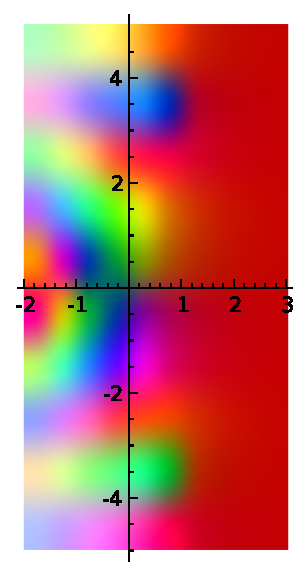
\includegraphics[width=.4\textwidth]{pics/27a-lser1.pdf}
\end{center}

As for the Riemann zeta function, there is a generalized Riemann
Hypothesis, which postulates that the nontrivials zeros of
$L(E,s)$ lie on a line, the line $\Re(s)=1$.
The first few imaginary parts of the nontrivial zeros of $L(E,s)$ are
\begin{lstlisting}
sage: L.zeros(5)
[4.04304401, 6.04893540, 8.21765037, 9.42919921, 10.9087283]
\end{lstlisting}


\section{The abc Conjecture}
The abc conjecture
concerns triples of coprime positive integers $a,b,c$  such that
$$
a+b = c.
$$
The {\em radical} of an integer $n$ is the product
of the distinct prime divisors of $n$, and the radical
of an abc triple $a,b,c$ is $r=r(a,b,c)=r(abc)$.
For example,
$$
  1 + 8 = 9
$$
has radical $r=2\cdot 3=6$.

\begin{conjecture}[Masser-Oesterl\'{e}]\label{conj:abc}
For every $\eps>0$ there are only finitely many
triples $a,b,c$ of coprime positive integers such
that $a+b=c$ and $r^{1+\eps}<c$,
where $r=r(a,b,c)$.
\end{conjecture}

Given $a,b$ it is trivial to find $c$ with $c=a+b$, and
usually the radical $r=r(a,b,c)$ is going to be bigger
than $c$.   A typical example is $a=4$, $b=15$.
We have $c=4+15=19$, and the radical is
$$2\cdot 3\cdot5\cdot19=570 \gg 19.$$

Now suppose for the moment that we have a counterexample
to Fermat's Last Theorem (see Section~\ref{sec:fltintro} above),
say
$$
 A^n + B^n = C^n,
$$
with $A,B,C$ coprime positive integers and $n\ge 5$ (say).
Letting $a=A^n, b=B^n, c=C^n$, we have
$$
r(a,b,c) = r(A^n,B^n,C^n) = r(A,B,C) = ABC <C^3 < C^n=c.
$$
According to Conjecture~\ref{conj:abc} (with
any choice of $\eps$), there can be only finitely many such
$(A,B,C)$.  In particular, Conjecture~\ref{conj:abc} implies
Fermat's Last Theorem for all sufficiently large $n$.
\footnote{An accepted proof of FLT is known (due to Wiles). There
is no accepted proof of ABC, but there is a claimed one,
which may or may not be right...
\begin{quote}
``The problem with wrong proofs to correct statements is that it is hard to give a counterexample.'' -- Hendrik Lenstra, \url{http://www.ucs.louisiana.edu/~avm1260/lenstra.html}
\end{quote}}

There's much computational work that goes into understanding
and refining the ABC conjecture.  For example,
Lenstra defined a notion of the {\em quality} of
a triple $a+b=c$ to be
$$q(a,b,c) = \frac{\log(c)}{\log(r(a,b,c))}.$$
As mentioned above, this number is usually very small, since
$r$ is typically much bigger than $c$.
However, there are some known triples $a,b,c$ of
high quality, but the ABC conjecture asserts there aren't too
many.  In fact, here is an equivalent version of the ABC conjecture:
\begin{conjecture}
For every $h>1$ there are only finitely many triples
$a,b,c$ with quality bigger than $h$.
\end{conjecture}

The highest quality triple ever found\footnote{See \url{http://www.math.leidenuniv.nl/~desmit/abc/}.} is
$$
   2 + 3^{10}\cdot 109 = 23^5,
$$
where
$$
q(a,b,c) = \frac{\log(23^5)}{\log(2\cdot 3 \cdot 109 \cdot 23)}
    = 1.62991168412\ldots
$$


\section{Public-key Cryptography}


\begin{quote}
``Nowadays, when a Number Theorist applies for a grant, he says
that Number Theory is used in cryptography, and so doing Number
Theory is good for National Security. Back then, since it was
before the discovery of America, they said Number Theory is
used in music. But I won't comment on the progress of
civilization since then.''\\-- Hendrik Lenstra, \url{http://www.ucs.louisiana.edu/~avm1260/lenstra.html}
\end{quote}



\chapter{Prime Numbers}

Main unsolved problem: the Riemann Hypothesis



\section{Infinitely many primes}
\section{The Prime number theorem}
\section{The Riemann hypothesis}
\section{The Explicit Formula}
\section{Generalizations to number fields}


\chapter{Arithmetic of Number Fields}
Main unsolved problem: class number 1 fields

\section{Class groups}
\section{The Gauss class number problem}
\section{Number fields of class number 1}
 (Cohen-lenstra, Bharghava)



\chapter{Diophantine Equations: Fermat and ABC}
Main unsolved problem: ABC conjecture

\section{Fermat's Last Theorem}
\section{The ABC Conjecture}
\section{Generalized Fermat equations}



\chapter{Elliptic Curves}
Important unsolved problem: the BSD conjecture (computing Mordell-Weil groups)

\section{The Group law}
\section{The Mordell-Weil theorem}
\section{Mazur's classification of torsion subroups}
\section{The $L$-series}
analytic continuation and functional equation (modularity)
\section{The Birch and Swinnerton-Dyer conjecture}
\section{The Hasse bound}
\section{The Explicit Formula}



\chapter{Modular Forms}
Important unsolved problem: modularity of elliptic curves
over totally real fields

\section{Ramanujan bound}
\section{Galois representations attached to modular forms}
\section{Modularity of elliptic curves}




\chapter{Public-key Cryptography}

Important unsolved problem: how difficult is the discrete log problem?

\section{Protocols: Diffie-Hellman, RSA, ElGamal, ...}
\section{Discrete log problem (baby-step, giant-step)}



\end{document}

%sagemathcloud={"zoom_width":145}